%----------------------------------------------------------------------------------------
%	PACKAGES AND THEMES
%----------------------------------------------------------------------------------------
\documentclass[aspectratio=43,xcolor=svgnames]{beamer} %dvipsnames o svgnames
\usetheme{Padova}
\usepackage{multicol}
\usepackage{hyperref}
\usepackage{graphicx} % Allows including images
\usepackage{booktabs} % Allows the use of \toprule, \midrule and \bottomrule in tables
%\usepackage{movie15}
\usepackage{tikz}
\usepackage{listings}
\usepackage{comment}
%\usepackage{xmpmulti}
%\usepackage{animate}
\usepackage{adjustbox}
%\usepackage{algorithm}
%\usepackage{algorithmic}
\usepackage{physics}
\usepackage{float}
\usepackage{caption}
\usepackage{subcaption}
\usepackage{comment}

\usepackage[
    backend=biber,
    style=numeric,%authoryear,%se no numeric. Questo è per cambiare cosa spunti alla fine
    %bibencoding=ascii,
    citestyle=numeric,%authoryear,%se no numeric. Questo cambia cosa si veda nel testo %se no alphabetic in entrambi
    sorting=nyt %sort by name, year,title
]{biblatex}

\addbibresource{bibliography.bib} %Imports bibliography file

\newcommand{\highlightred}[1]{%
  \colorbox{red!50}{$\displaystyle#1$}}
\newcommand{\highlightgreen}[1]{%
  \colorbox{green!50}{$\displaystyle#1$}}

%%%% Tikz related stuff %%
\usepackage{import}
%\subimport{./plotter}{init}
\usetikzlibrary{positioning}
\usetikzlibrary{3d} %for including external image 

\def\Blank{rgb:white,4}
\def\ConvColor{rgb:yellow,5;red,2.5;white,5}
\def\ConvReluColor{rgb:yellow,5;red,5;white,5}
\def\PoolColor{rgb:red,1;black,0.3}
\def\DcnvColor{rgb:blue,5;green,2.5;white,5}
\def\DcnvReluColor{rgb:blue,5;green,5;white,5}
\def\SoftmaxColor{rgb:blue,5;red,2.5;white,5}
\def\SumColor{rgb:blue,5;green,15}
%----------------------------------------------------------------------------------------
%	TITLE PAGE
%----------------------------------------------------------------------------------------

% The title
\title[shorttitle]{Emulating Cosmological Likelihoods with Machine Learning}
\subtitle{\textit{MSc in Physics of Data}} % o Master Thesis in Physics of Data
% \subtitle{A new approach to cosmological inference acceleration via emulation \\
%           \textit{MSc in Physics of Data}}

% oppure Master Candidate
\author{\emph{MSc Candidate:} Marco Giunta\\
        \emph{Supervisor:} Michele Liguori (UniPD)\\
        \emph{Co-Supervisor:} Marco Raveri (UniGE)
        }
%\institute[NTU] % Your institution may be shorthand to save space
{
    % Your institution for the title page
    %Università degli studi di Padova
    %\vskip 3pt
}
%\date{\today} % Date, can be changed to a custom date
\date{7 September 2023}

\AtBeginSection[]
{
  \begin{frame}
    \small
    \frametitle{Overview}
    \tableofcontents[currentsection]
  \end{frame}
}
%----------------------------------------------------------------------------------------
%	PRESENTATION SLIDES
%----------------------------------------------------------------------------------------

\begin{document}

\begin{frame}
    % Print the title page as the first slide
    \titlepage
\end{frame}

\begin{frame}{Overview}
    \small
    \tableofcontents % necessario?
\end{frame}



%%%%%%%%%%%%%%%%%%%%%%%%%%%%%%%%%%%%%%%%%%%%%%%%%%%%
%%%%%%%%%%%%%%%%%%%%%%%%%%%%%%%%%%%%%%%%%%%%%%%%%%%%

\section{Inference Acceleration via Emulators in Cosmology}

\begin{comment}
\begin{frame}{CMB-based inference: Power Spectrum}
    \begin{figure}[H]
        \centering
        \includegraphics[width=0.7\textwidth]{img/Planck_CMB2018.jpg}
        \caption{CMB temperature anisotropy field.}
        %\label{fig:enter-label}
    \end{figure}
    \pause % conta come 1, quindi devo posticipare i numeri
    % https://latex-beamer.com/faq/uncover-formula/
    The CMB field is a Gaussian Process:
    \only<2>{
    \begin{equation*}
        \ln\mathcal{L}(D|\theta)\propto (\hat{C}_\ell(D) - C_\ell(\theta))^T \Sigma^{-1}(\hat{C}_\ell(D) - C_\ell(\theta))
    \end{equation*}
    }
    \only<3>{
    \begin{equation*}
        \ln\mathcal{L}(D|\theta)\propto (\highlightred{\hat{C}_\ell(D)} - C_\ell(\theta))^T \Sigma^{-1}(\hat{C}_\ell(D) - C_\ell(\theta))
    \end{equation*}
    }
    \only<4>{
    \begin{equation*}
        \ln\mathcal{L}(D|\theta)\propto (\highlightred{\hat{C}_\ell(D)} - \highlightgreen{C_\ell(\theta)})^T \Sigma^{-1}(\hat{C}_\ell(D) - C_\ell(\theta))
    \end{equation*}
    }
    \pause %https://tex.stackexchange.com/questions/116913/display-the-definition-of-each-items-in-beamer-one-by-one-using-onslide-or-any-m
    \begin{itemize}
        \item<3-> $\highlightred{\hat{C}_\ell(D)}$: dataset dependent (fixed)
        \item<4-> $\highlightgreen{C_\ell(\theta)}$: parameter dependent (variable)
    \end{itemize}
\end{frame}
\end{comment}

\begin{frame}{CMB Temperature Anisotropy Field}
    \begin{figure}[H]
        \centering
        \includegraphics[width=0.7\textwidth]{img/Planck_CMB2018.jpg}
        \caption{CMB temperature anisotropy field.}
        %\label{fig:enter-label}
    \end{figure}
    \pause
    \begin{itemize}[<+->]
        \item Temperature differences are due to quantum fluctuations in the early universe, and are thus random in nature
        \item Their statistical properties are described by the \emph{CMB power spectrum} $C_\ell(\theta)$, a compressed equivalent representation
    \end{itemize}
\end{frame}
\begin{comment}
\begin{frame}{CMB-based inference}
    % https://latex-beamer.com/faq/uncover-formula/
    By computing the power spectrum for parameters $\Tilde{\theta}$ and comparing it with the \emph{observed} spectrum we can evaluate how likely $\Tilde{\theta}$ is.
    \only<2>{
    The CMB field is a Gaussian Process:
    \begin{equation*}
        \ln\mathcal{L}(D|\theta)\propto (\hat{C}_\ell(D) - C_\ell(\theta))^T \Sigma^{-1}(\hat{C}_\ell(D) - C_\ell(\theta))
    \end{equation*}
    }
    \only<3>{
    \begin{equation*}
        \ln\mathcal{L}(D|\theta)\propto (\highlightred{\hat{C}_\ell(D)} - C_\ell(\theta))^T \Sigma^{-1}(\hat{C}_\ell(D) - C_\ell(\theta))
    \end{equation*}
    }
    \only<4>{
    \begin{equation*}
        \ln\mathcal{L}(D|\theta)\propto (\highlightred{\hat{C}_\ell(D)} - \highlightgreen{C_\ell(\theta)})^T \Sigma^{-1}(\hat{C}_\ell(D) - C_\ell(\theta))
    \end{equation*}
    }
    \pause %https://tex.stackexchange.com/questions/116913/display-the-definition-of-each-items-in-beamer-one-by-one-using-onslide-or-any-m
    \begin{itemize}
        \item<3-> $\highlightred{\hat{C}_\ell(D)}$: dataset dependent (fixed during posterior sampling)
        \item<4-> $\highlightgreen{C_\ell(\theta)}$: parameter dependent (variable during posterior sampling)
    \end{itemize}
\only<5>{
\begin{figure}[H]
    \centering
    \includegraphics[width=0.5\textwidth]{img/Planck_cmb_density.png}
    \caption{Comparison between observed and theoretical CMB power spectrum for multiple CDM density values.}
    %\label{fig:enter-label}
\end{figure}
}
\end{frame}
\end{comment}

\begin{frame}{CMB Power Spectrum}
    % https://latex-beamer.com/faq/uncover-formula/
    By computing the power spectrum for parameters $\Tilde{\theta}$ and comparing it with the \emph{observed} spectrum we can evaluate how likely $\Tilde{\theta}$ is:
    \begin{figure}[H]
        \centering
        \includegraphics[width=0.7\textwidth]{img/Planck_cmb_density.png}
        \caption{Comparison between observed and theoretical CMB power spectrum for multiple CDM density values.}
        %\label{fig:enter-label}
    \end{figure}
\end{frame}
\begin{frame}{CMB-based Inference}
    To use the CMB to obtain a Bayesian posterior over $\theta$ values we need to evaluate how likely each theoretical power spectrum is given the observed one.
    \pause

    
    The CMB field is a \emph{Gaussian Process}:
    \only<2>{
    \begin{equation*}
        \ln\mathcal{L}(D|\theta)\propto (\hat{C}_\ell(D) - C_\ell(\theta))^T \Sigma^{-1}(\hat{C}_\ell(D) - C_\ell(\theta))
    \end{equation*}
    }
    \only<3>{
    \begin{equation*}
        \ln\mathcal{L}(D|\theta)\propto (\highlightred{\hat{C}_\ell(D)} - C_\ell(\theta))^T \Sigma^{-1}(\hat{C}_\ell(D) - C_\ell(\theta))
    \end{equation*}
    }
    \only<4>{
    \begin{equation*}
        \ln\mathcal{L}(D|\theta)\propto (\highlightred{\hat{C}_\ell(D)} - \highlightgreen{C_\ell(\theta)})^T \Sigma^{-1}(\hat{C}_\ell(D) - C_\ell(\theta))
    \end{equation*}
    }
    \pause %https://tex.stackexchange.com/questions/116913/display-the-definition-of-each-items-in-beamer-one-by-one-using-onslide-or-any-m
    \begin{itemize}
        \item<3-> $\highlightred{\hat{C}_\ell(D)}$: dataset dependent (fixed during posterior sampling)
        \item<4-> $\highlightgreen{C_\ell(\theta)}$: parameter dependent (variable during posterior sampling)
    \end{itemize}
\end{frame}

\begin{frame}{Cosmological Emulators}
    \begin{itemize}[<+->]
        \item To infer the value of cosmological parameters we need to compare an experimentally measured quantity (e.g. $\hat{C}_\ell(D)$) with the value of that same quantity predicted theoretically assuming a certain choice of the cosmological parameters/model (e.g. $C_\ell(\theta)$); \emph{this is a general property of cosmological inferences, i.e. it always holds.}
        \item Theoretical predictions (e.g. $C_\ell(\theta)$) can be computed exactly using expensive specialized solvers, which are usually the computational bottleneck in inference pipelines
        \item For this reason it makes sense to train an \emph{emulator}, i.e. a machine learning model that replaces the expensive exact computation; this is possible because e.g. the mapping $\theta \mapsto C_\ell$ is smooth
        \item Common procedure: train an emulator valid under certain assumptions, then publish it
    \end{itemize}
\end{frame}

\begin{frame}{Shortcomings of the Out-of-the-box Approach}
In order to use a pre-existing emulator to accelerate parameter inference several requirements must be met:
\pause
\begin{itemize}[<+->]
    \item appropriate cosmological likelihood/model
    \item required accuracy
    \item suitable ML model/preprocessing
\end{itemize}
\pause
\vspace{1.5em}
If any of these conditions do not hold then a custom emulator must be trained from scratch; this means trading \emph{computer time} for \emph{human time}, which negates the time benefit of using emulators...
\pause
\vspace{0.7em}


...unless the process of implementing an emulator can be \emph{automated}!
\pause
In particular we propose a \emph{change of paradigm}: we replace prebuilt emulators with DIY ones, which are to be trained using a standardized, fully automated procedure
\end{frame}

\section{\textsc{CosmoLIME}: A New Approach To Emulation}
\begin{frame}{Introducing CosmoLIME}
We introduce \textsc{CosmoLIME}, the \emph{Cosmological Likelihood Machine learning Emulator}, to automate the process of building custom emulators.

\vspace{1em}
Relevant features include:
\pause
\begin{itemize}[<+->]
    \item fully automated data generation and ML model training
    \item support for arbitrary likelihood functions/cosmological models
    \item support for arbitrary ML models/preprocessing
    \item support for automated testing
    \item other useful tools (logging, model caching, etc.)
\end{itemize}
\end{frame}

\begin{frame}{Implementing An Emulator With CosmoLIME}
% 3 step process: lista
% standard regression ma possiamo generare dati infiniti e senza rumore perché f e nota
In general training an emulator from scratch is a three-step process:
\pause
\begin{itemize}[<+->]
    \item obtain a suitable training dataset
    \item train the ML model of choice
    \item test the result via accuracy metrics/statistical tests
\end{itemize}
\pause
\vspace{1em}
A training dataset of arbitrarily many, noise-free samples can be obtained using the available exact solvers; the remaining tasks are solved as usual in regression problems. This means that \textsc{CosmoLIME} must automate both the data generation and the model optimization.
\end{frame}

\begin{frame}{CosmoLIME Software Hierarchy}
\begin{figure} % prova a imitare il disegno di Luca
    \centering
    %\includegraphics{}
    \resizebox{30em}{!}{ % \resizebox scala la figura orizzontalmente/verticalmente, \scalebox = unico fattore
    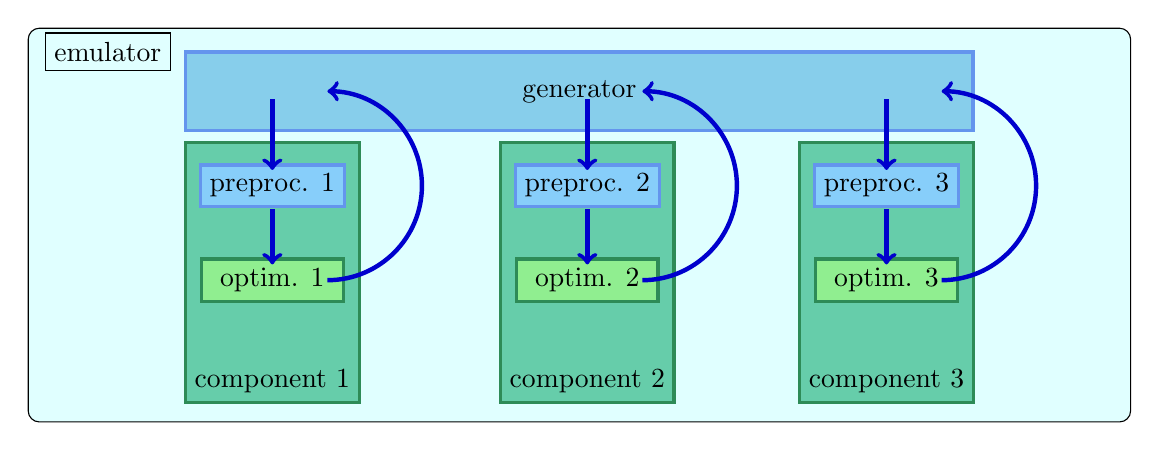
\begin{tikzpicture}[
    gennode/.style={rectangle, draw=CornflowerBlue, fill=SkyBlue, very thick, minimum height=10mm, minimum width=100mm},
    ppnode/.style={rectangle, draw=CornflowerBlue, fill=LightSkyBlue, very thick, minimum size=5mm},
    optnode/.style={rectangle, draw=SeaGreen, fill=LightGreen, very thick, minimum width=18mm},
    compnode/.style={rectangle, draw=SeaGreen, fill=MediumAquamarine, very thick, minimum height=30mm, minimum width=10mm, text height=30mm},
    ]
      \uncover<1->{
      \draw[rounded corners, black, fill=LightCyan] (0, 0) rectangle (14, 5) {};
      \node[draw] at (1.01, 4.7) {emulator}; % aggiungi il testo sopra direttamente^
      }
      \uncover<2->{ % partial reveal
      \node[gennode] (maintopic) at (7, 4.2) {generator}; % specificarne la posizione?
      }
      % prima componente
      \uncover<3->{
      \node[compnode] at (3.1, 1.9) {component 1};
      \node[ppnode] at (3.1, 3) {preproc. 1};
      \node[optnode] at (3.1, 1.8){optim. 1};
      }
      
      \draw<4->[ultra thick, ->, color=MediumBlue] (3.1, 4.1) -- (3.1, 3.2);      
      \draw<5->[ultra thick, ->, color=MediumBlue] (3.1, 2.7) -- (3.1, 2.0);
      \draw<6->[ultra thick, ->, color=MediumBlue] (3.8, 1.8) arc (-90:90:1.2);

      % altre componenti
      \uncover<7->{
      \node[compnode] at (7.1, 1.9) {component 2};
      \node[ppnode] at (7.1, 3) {preproc. 2};
      \node[optnode] at (7.1, 1.8){optim. 2};
      \draw[ultra thick, ->, color=MediumBlue] (7.1, 4.1) -- (7.1, 3.2);
      \draw[ultra thick, ->, color=MediumBlue] (7.1, 2.7) -- (7.1, 2.0);
      \draw[ultra thick, ->, color=MediumBlue] (7.8, 1.8) arc (-90:90:1.2);
      }
      \uncover<8->{
      \node[compnode] at (10.9, 1.9) {component 3};
      \node[ppnode] at (10.9, 3) {preproc. 3};
      \node[optnode] at (10.9, 1.8){optim. 3};
      \draw[ultra thick, ->, color=MediumBlue] (10.9, 4.1) -- (10.9, 3.2);
      \draw[ultra thick, ->, color=MediumBlue] (10.9, 2.7) -- (10.9, 2.0);
      \draw[ultra thick, ->, color=MediumBlue] (11.6, 1.8) arc (-90:90:1.2);
      }
    \end{tikzpicture}
    }
    \caption{Schematic representation of \textsc{CosmoLIME}.}
    \label{fig:cosmolime_schematics}
\end{figure}
\end{frame}





\section{Example: Discovering Dark Energy}
\begin{frame}{Dark Energy Simplified Model}
As a simple application we can prove the existence of dark energy using \textsc{CosmoLIME}. We use the standard $\Lambda$-CDM cosmological model with all parameters fixed to their fiducial values, except for \emph{relative matter density} and \emph{relative dark energy density}:
\begin{equation*}
    \Omega_m \equiv \frac{\rho_m}{\rho_{\text{tot}}}, \quad \Omega_{\text{DE}} \equiv \frac{\rho_{\text{DE}}}{\rho_{\text{tot}}} \quad \text{with} \quad \Omega_m+\Omega_{\text{DE}} = 1
\end{equation*}
\pause
Then the problem of whether dark energy exists becomes equivalent to asking whether $\Omega_m=1$ or $\Omega_m\neq 1$; this means we have a simple 1-parameter model, making inference trivial.
\end{frame}

\begin{frame}{Type Ia Supernovae}
\only<1>{
In this simplified model the $\Omega_m$ parameter is the only quantity influencing the \emph{luminosity distances of type Ia supernovae}, which are normally distributed around:
\begin{equation*}
    D_L(z) = D_0(1+z)\int_0^z \frac{\dd{x}}{\sqrt{\Omega_m(1+x)^3+\Omega_{\text{DE}}}}
\end{equation*}
\begin{equation*}
    \mu(z)\equiv 5\log_{10}D_L(z)
\end{equation*}
}
\only<2>{
\begin{figure}[H]
    \centering
    \includegraphics[width=0.9\textwidth]{img/sn_data.pdf}
    \caption{Observed/predicted $\mu(z)/\mu(0)$ assuming $\Omega_m=1$ or $\Omega_m=0.3$.}
    %\label{fig:enter-label}
\end{figure}
}
\end{frame}

\begin{frame}{Inferring $\Omega_m$}
By observing an experimental dataset $\{z_n, \hat{\mu}(z_n)\}$ we perform inference by exploiting the fact that \emph{distances are distributed according to a Gaussian}:
\begin{equation*}
    \ln\mathcal{L}(\hat{\mu}|\mu, \Sigma) \propto (\mu-\hat{\mu})^T\Sigma^{-1}(\mu-\hat{\mu})
\end{equation*}
\pause
Marginalizing w.r.t. nuisance parameter $D_0$:
\begin{equation*}
    \ln\mathcal{L}_m(\hat{\mu}|\mu, \Sigma) \propto -\frac{1}{2}(\mu-\hat{\mu})^T\Sigma^{-1}(\mu-\hat{\mu})+\frac{1}{2}\frac{\left[(1)\Sigma^{-1}(\hat{\mu}-\mu)\right]^2}{(1)\Sigma^{-1}(1)}
\end{equation*}
By emulating this likelihood with \textsc{CosmoLIME} and using a uniform prior for simplicity we can obtain the $\Omega_m$ posterior.
\end{frame}
\begin{frame}{Inference Results}
\only<1>{
\begin{figure}[H]
    \centering
    \includegraphics[width=0.95\textwidth]{img/loglikelihood_dt.pdf}
    \caption{Exact vs emulated marginalized log-likelihood.}
    %\label{fig:enter-label}
\end{figure}
}
\only<2>{
\begin{figure}[H]
    \centering
    \includegraphics[width=0.95\textwidth]{img/posterior_dt.pdf}
    \caption{Exact vs emulated $\Omega_m$ posterior.}
    %\label{fig:enter-label}
\end{figure}
}
\only<3>{
We notice that the posterior has a strong peak in $\Omega_m\approx 0.3$, thus implying that about $\sim 70\%$ of the ``stuff'' in our universe is dark energy.
Rigorous probabilistic statements can be obtained by normalizing the posterior (e.g. via direct numerical integration in this simple example).


In particular we find
\begin{equation*}
    \Omega_m = 0.298\pm 0.043 \ \text{(MAP $\pm$ $68\%$ cred. int.)}
\end{equation*}
without significant differences between using the exact or emulated posterior, and in good agreement with the currently accepted value.
}
\only<4>{
\begin{figure}[H]
    \centering
    \includegraphics[width=0.95\textwidth]{img/cred_intervals.pdf}
    \caption{Posterior credibility intervals.}
    %\label{fig:enter-label}
\end{figure}
}
\end{frame}

\begin{frame}{Bayesian Model Comparison}
Another way to infer the existence of dark energy from this data is to perform \emph{Bayesian model comparison} between model $M_0$ ($\Omega_m=1$ exactly) and model $M_1$ ($\Omega_m \in [0, 1]$) using e.g. a uniform prior on models:
\pause
\begin{equation*}
    \frac{P(M_1|D)}{P(M_0|D)} = \frac{P(D|M_1)}{P(D|M_0)} \equiv\frac{E_1}{E_0}
\end{equation*}
\pause
$E_1$ is the evidence of the $\Omega_m$ posterior; $E_0=P(\Omega_m=1|D)$, i.e. $E_0$ equals the posterior in $\Omega_m=1$.
\pause
With or without the emulator we find:
\begin{equation*}
    \ln(E_1/E_0) = \ln E_1 - \ln E_0 \approx 239
\end{equation*}
which means that \emph{a universe with dark energy is strongly preferred even accounting for the Occam penalty (at least according to this data)}.
\end{frame}


\section{Conclusions And Future Work}
\begin{frame}{Thesis Summary}
\begin{itemize}[<+->]
    \item Cosmological emulators are ML models that can be used to accelerate inference pipelines by replacing the expensive exact evaluations; unless a suitable prebuilt emulator is available this requires training the model from scratch, which can ruin the chance to actually save time to perform inferences.
    \item To solve this we proposed a change of paradigm: from prebuilt to DIY emulators. This is achieved with \textsc{CosmoLIME}, the \emph{Cosmological Likelihood Machine learning Emulator}: a model-agnostic, self-training, machine learning-based framework to emulate arbitrary likelihood functions in a fully automated way.
    \item To design such a framework we simply need to automate a slightly modified version of the standard regression problem; we applied these results to simple but realistic examples.
\end{itemize}
\end{frame}
\begin{frame}{Future Challenges}
Even though \textsc{CosmoLIME} already works several features may be added to make it truly compelling to the astrophysical community:
\pause
\begin{itemize}[<+->]
    \item \textsc{CosmoLIME} has yet to be tested on serious problems; a good starting point would be to reproduce prebuilt research-ready emulators, showing how they can be reproduced with minimum effort.
    \item More statistically sound accuracy metrics are needed; simple ML metrics can lead to overconfident models, whose optimization is prematurely stopped and results in e.g. biased posteriors.
    \item Further technical improvements can make \textsc{CosmoLIME} more enticing (better logging, complete parallelization, etc.).
\end{itemize}
\only<5>{
Achieving these points can turn \textsc{CosmoLIME} into a publication-ready framework.
}
\end{frame}


\end{document}